\begin{frame}{Introduction}
	The Capacitated Vehicle Routing Problem (\textbf{CVRP}) \parencite{dantzig1959}
	is an \textcolor{blue}{NP-hard combinatorial optimization routing problem} with applications in \textcolor{blue}{logistics} (transportation, distribution, delivery).

	\vspace{0.25cm}

	\begin{columns}

		\begin{column}{.35\textwidth}
			\onslide<+->{
				\centering
				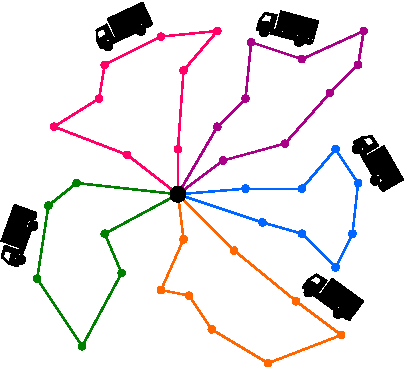
\includegraphics[height=4cm]{Imgs/CVRP-example.cropped.pdf}
			}
		\end{column}
		\begin{column}{.65\textwidth}
			\onslide<+->{
				\begin{itemize}[<+->]
					\item CVRP defined on a complete graph. We are given:
					      \begin{itemize}[<.->]
						      \item The amount of \textcolor{blue}{available vehicles} with their \textcolor{blue}{capacity}.
						      \item A \textcolor{blue}{central depot} where vehicles are stationed.
						      \item Customers' \textcolor{blue}{locations}.
						      \item The \textcolor{blue}{demands} of the individual customers.
					      \end{itemize}

					\item Objective:
					      \begin{itemize}[<.->]
						      \item \textcolor{red}{Minimize overall routing costs while meeting the needs of \textbf{all} customers.}
					      \end{itemize}
				\end{itemize}
			}
		\end{column}
	\end{columns}
\end{frame}

\begin{frame}{Branch-price-and-cut}
	\begin{columns}
		\begin{column}{.7\textwidth}
			\begin{itemize}[<+->]
				\item \textcolor{blue}{Branch-price-and-cut} (BPC) is an \textbf{exact approach} for solving combinatorial optimization problems.
				      \begin{itemize}
					      \item It is an extension of traditional \textcolor{blue}{branch-and-cut} (BAC) frameworks.
					      \item State-of-the-art VRP solvers in the last two decades \parencite{gutierrez-jarpa2010, archetti2011, bettinelli2011, contardo2014, contardo2015, pecin2017new, pecin2017improved, pessoa2020generic}.
					            \pause[\thebeamerpauses]
					      \item Compared to traditional BAC frameworks, can tackle \textbf{huge} \textcolor{blue}{mixed integer programming} models described by exponential amounts of decision variables.
				      \end{itemize}
			\end{itemize}
		\end{column}
		\begin{column}{.3\textwidth}
			{
				\fontsize{9.5pt}{9.5pt}\selectfont

				\begin{align*}
					\min_{\lambda} \quad z_\mt{SC}(\lambda) & = \sum_{p \in P}  c_p \lambda_p                                      \\
					                                        & \sum_{p \in P} \lambda_{p} = K                                       \\
					                                        & \sum_{p \in P}  a_{ip} \lambda_p \ge 1       \quad \forall i \in V_0 \\
					                                        & \lambda_p                    \in \Set*{0, 1} \quad \forall p \in P.
				\end{align*}
			}
		\end{column}
	\end{columns}

	\pause[\thebeamerpauses]

	\begin{itemize}[<+->]
		\item \textcolor{red}{How?}
		      \begin{itemize}
			      \item \textcolor{blue}{Column Generation} (CG): decision variables are generated lazily.
			            \begin{itemize}
				            \item In VRP, decision variables represent \textcolor{blue}{single vehicle feasible routes}.
			            \end{itemize}
			      \item \textcolor{red}{\textbf{Pricing}} in CVRP, is the art of feeding the BPC approach with good reduced cost routes to bring it towards fast optimality convergence.
		      \end{itemize}
	\end{itemize}
\end{frame}

\begin{frame}{Contemporary Approaches for Pricing}
	\onslide<+->{

		\begin{itemize}[<+->]
			\item Pricing Problem (PP) in its "natural" form is an \textbf{NP-hard} combinatorial optimization problem \parencite{dror1994}.
			      \begin{itemize}[<.->]
				      \item \textcolor{olive}{Relaxation} of the pricing problem to make it solvable in \textcolor{blue}{pseudo-polynomial time}.
			      \end{itemize}
			\item \textcolor{blue}{Dynamic programming} algorithms (exact and heuristics) to solve the \textcolor{olive}{relaxed} PP:
			      \begin{itemize}[<.->]
				      \item \textbf{labeling algorithm} proposed in \textcite{desrochers1992,feillet2004}
			      \end{itemize}

		\end{itemize}
	}

	\vspace{0.5cm}

	\onslide<+->{

		\begin{itemize}
			\item \textcolor{red}{\textbf{Two major issues with contemporary approaches}}:
			      \begin{enumerate}[<+->]
				      \item (weak) \textcolor{olive}{relaxing} the PP worsens the dual bounds fed to the BPC (increasing column generation time).
				            \begin{itemize}[<.->]
					            \item \textcolor{blue}{Improved in last decade} thanks to "smart" relaxations \parencite{baldacci2011}.
				            \end{itemize}
				      \item (strong) \textbf{Labeling} algorithm's performance degrades as the \textcolor{blue}{vehicle capacity increases} (longer routes), limiting its applicability to modern distribution problems.
			      \end{enumerate}
		\end{itemize}
	}
\end{frame}

\begin{frame}{Contributions}
	\begin{columns}
		\begin{column}{0.3\textwidth}
			\centering
			
\includegraphics[width=\textwidth]{./Imgs/idea.png}
		\end{column}
		\begin{column}{0.7\textwidth}
			\begin{enumerate}
				\item An exact \textcolor{blue}{branch-and-cut} approach for the \textcolor{olive}{\textbf{non}-relaxed} pricing problem.
				      \begin{itemize}
					      \item Almost no works on this domain, except \parencite{jepsen2014}.
				      \end{itemize}
				\item Verify its competitiveness at solving the PP as the \textcolor{blue}{vehicle capacity increases}.
			\end{enumerate}
		\end{column}
	\end{columns}
\end{frame}

\begin{frame}{Implementation}
	\begin{columns}
		\begin{column}{.85\textwidth}
			\onslide<+->{

				\begin{itemize}
					\item Branch-and-cut implementation based on the \textcolor{blue}{IBM ILOG CPLEX optimizer}.
					\item The \textbf{Capacitated Profitable Tour Problem} (CPTP) \parencite{jepsen2014} was used as the base IP formulation.
					\item Implemented in \texttt{C} and available online\footnote[1]{\url{https://github.com/dparo/master-thesis}} under a permissive license.

				\end{itemize}
			}

			\vspace{0.5cm}

			\onslide<+->{
				\begin{itemize}
					\item Some implementation details:
					      \begin{itemize}
						      \item Separation of \textcolor{blue}{cutting-planes} both for integral and fractional solutions: GSEC, RCC, GLM.
						      \item Push relabel max-flow and Gomory-Hu trees employed for fractional separation.
					      \end{itemize}
				\end{itemize}
			}
		\end{column}
		\begin{column}{0.15\textwidth}
			\centering
			
\includegraphics[width=\textwidth]{./Imgs/IBM-ILOG-CPLEX-logo.png}
		\end{column}
	\end{columns}
\end{frame}

\begin{frame}{Empirical evaluation}
	\begin{columns}
		\begin{column}{0.2\textwidth}
			\centering
			
\includegraphics[width=\textwidth]{./Imgs/testing.png}
		\end{column}
		\begin{column}{0.8\textwidth}
			\begin{itemize}
				\item We've modified the commonly employed traditional instances proposed in
				      \cite{dantzig1959, christofides1969, gaskell1967bases, gillett1974heuristic,christofides1979vehicle,fisher1994,augerat1995}.

				\item Running time measured through \textbf{performance profiles} \parencite{dolan2002}.
			\end{itemize}
		\end{column}
	\end{columns}
\end{frame}

\begin{frame}{Results (1/2)}

\end{frame}

\begin{frame}{Results (2/2)}

\end{frame}

\begin{frame}{Conclusions and Future Work}
	The proposed branch-and-cut pricer proved competitive at solving some PP:
	\begin{itemize}
		\item \textcolor{blue}{Branch-and-cut} approaches may supplement the traditional \textcolor{blue}{labeling algorithm}.
		\item Suggesting future research on \textcolor{blue}{branch-and-cut} approaches in the context of \textbf{pricing for the CVRP}.
		      Benefits:
		      \begin{itemize}
			      \item Improve performance of contemporary CVRP solvers.
		      \end{itemize}
	\end{itemize}
\end{frame}

\begin{frame}{The end}
	\begin{center}
		\begingroup
		\fontsize{18pt}{18pt}\selectfont
		Thank, you.
		\endgroup
	\end{center}
\end{frame}

\appendix

\begin{frame}
\end{frame}

\begin{frame}
	\begin{center}
		\begingroup
		\fontsize{18pt}{18pt}\selectfont
		Additional material.
		\endgroup
	\end{center}
\end{frame}

\begin{frame}{Integer Programming}
	MIP solvers are rather general and can be used to solve a wide range of problems from various fields \parencite{bixby2007progress}.
	MIP models are, in spirit, a way to mathematically program a solver to achieve the desired solution.
	A MIP solver can solve a mixed-integer linear programming formulation
	expressed as \parencite{wolsey1999integer}:
	\begin{align}
		 & \max_{x, y} & c^T x + d^T y                                 \\
		 & \text{s.t.} & A x + B y \le b  \label{eq:general-mip-bound} \\
		 &             & x \in \R^n                                    \\
		 &             & y \in \Z_{+}^k,
	\end{align}
	where $A \in \R^{m \times n}, B \in \R^{m \times k}$ are matrices and
	$c \in \R^n, d \in R^k, b \in \R^m$ are vector coefficients.
	The bound in \cref{eq:general-mip-bound} can also be rewritten in equality and/or greater form.

\end{frame}

\begin{frame}{Set Covering formulation}
	Let $P = \Set*{p \mid p\ \text{is a single-truck elementary feasible route}}$ be the set of all feasible routes.

	\begin{align}
		\min_{\lambda} \quad z_\mt{SC}(\lambda) & = \sum_{p \in P}  c_p \lambda_p              & \label{eq:set-covering-obj-func}                                                       \\
		                                        & \sum_{p \in P} \lambda_{p} = K               & \label{eq:set-covering-K-routes}                                                       \\
		                                        & \sum_{p \in P}  a_{ip} \lambda_p \ge 1       & \quad \forall i \in V_0 \label{eq:set-covering-customers-visited-by-exactly-one-route} \\
		                                        & \lambda_p                    \in \Set*{0, 1} & \quad \forall p \in P \label{eq:set-covering-lambda-mip-var-bounds}.
	\end{align}
\end{frame}

\begin{frame}{The Pricing Sub-problem}
	To advance the column generation, the \textcolor{blue}{pricer}, a critical component in BPC frameworks, needs to solve the \textcolor{blue}{pricing sub-problem} (PP):
	\begin{itemize}
		\item An \textcolor{blue}{Elementary Shortest Path Problem with Capacity Constraints} (\textbf{ESPPCC}) in a reduced cost network with negative cycles.
		      \begin{itemize}
			      \item NP-hard problem \parencite{dror1994}.
		      \end{itemize}
		\item \textbf{Relax elementarity condition} to make it solvable in pseudo-polynomial time:
		      \begin{itemize}
			      \item $q$-routes with 2-cycles elimination \parencite{christofides1969}.
			      \item $q$-routes with arbitrary $k$-cycles elimination \parencite{christofides1969}.
			      \item ng-routes \parencite{baldacci2011}.
		      \end{itemize}
		\item State-of-the-art solutions for the \textcolor{olive}{relaxed} PP are based on \textcolor{blue}{dynamic programming}:
		      \begin{itemize}
			      \item \textbf{labeling algorithm} \parencite{desrochers1992, feillet2004}.
		      \end{itemize}
	\end{itemize}
\end{frame}
